
\begin{cverbatim}
\begin{tikzpicture}
    \draw (-1.5, 0) -- (1.5, 0);
    \draw (0, -1.5) -- (0, 1.5);
\end{tikzpicture}
\end{cverbatim}

\begin{tikzpicture}
    \draw (-1.5, 0) -- (1.5, 0);
    \draw (0, -1.5) -- (0, 1.5);
\end{tikzpicture}

\begin{cverbatim}
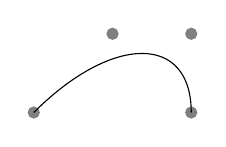
\begin{tikzpicture}
    \filldraw [gray] (0,0) circle (2pt)
                     (1,1) circle (2pt)
                     (2,1) circle (2pt)
                     (2,0) circle (2pt);
    \draw (0,0) .. controls (1,1) and (2,1) .. (2,0);
\end{tikzpicture}
\end{cverbatim}

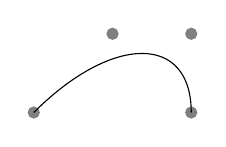
\begin{tikzpicture}
    \filldraw [gray] (0,0) circle (2pt)
                     (1,1) circle (2pt)
                     (2,1) circle (2pt)
                     (2,0) circle (2pt);
    \draw (0,0) .. controls (1,1) and (2,1) .. (2,0);
\end{tikzpicture}

\begin{cverbatim}
\begin{tikzpicture}
    \draw (-1.5,0) -- (1.5,0);
    \draw (0,-1.5) -- (0,1.5);
    \draw (-1,0) .. controls (-1,0.555) and (-0.555,1) .. (0,1)
                 .. controls (0.555,1) and (1,0.555) .. (1,0);
\end{tikzpicture}
\end{cverbatim}

\begin{tikzpicture}
    \draw (-1.5,0) -- (1.5,0);
    \draw (0,-1.5) -- (0,1.5);
    \draw (-1,0) .. controls (-1,0.555) and (-0.555,1) .. (0,1)
                 .. controls (0.555,1) and (1,0.555) .. (1,0);
\end{tikzpicture}

\begin{cverbatim}
\tikz \draw (0,0) circle (10pt);
\end{cverbatim}

\tikz \draw (0,0) circle (10pt);

\begin{cverbatim}
\tikz \draw (0,0) ellipse (20pt and 10pt);
\end{cverbatim}

\tikz \draw (0,0) ellipse (20pt and 10pt);

\begin{cverbatim}
\tikz \draw[rotate=30] (0,0) ellipse (20pt and 10pt);
\end{cverbatim}

\tikz \draw[rotate=30] (0,0) ellipse (20pt and 10pt);

\begin{cverbatim}
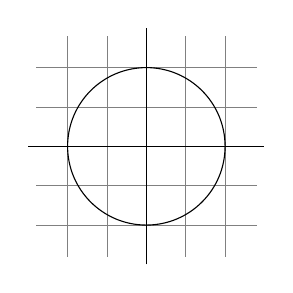
\begin{tikzpicture}
    \draw[step=.5cm, gray, very thin] (-1.4,-1.4) grid (1.4, 1.4);
    \draw (-1.5,0) -- (1.5,0);
    \draw (0,-1.5) -- (0,1.5);
    \draw (0,0) circle (1cm);
\end{tikzpicture}
\end{cverbatim}

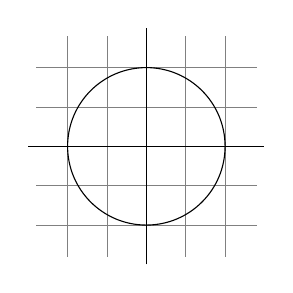
\begin{tikzpicture}
    \draw[step=.5cm, gray, very thin] (-1.4,-1.4) grid (1.4, 1.4);
    \draw (-1.5,0) -- (1.5,0);
    \draw (0,-1.5) -- (0,1.5);
    \draw (0,0) circle (1cm);
\end{tikzpicture}


\begin{cverbatim}
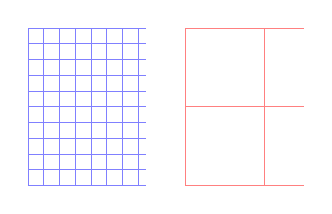
\begin{tikzpicture}
    [rui's grid/.style = {help lines, color=#1!50},
     rui's grid/.default = blue]
    \draw[step=.2cm, rui's grid] (0,0) grid (1.5,2);
    \draw[rui's grid=red] (2,0) grid (3.5,2);
\end{tikzpicture}
\end{cverbatim}

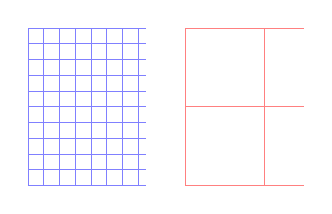
\begin{tikzpicture}
    [rui's grid/.style = {help lines, color=#1!50},
     rui's grid/.default = blue]
    \draw[step=.2cm, rui's grid] (0,0) grid (1.5,2);
    \draw[rui's grid=red] (2,0) grid (3.5,2);
\end{tikzpicture}

\begin{cverbatim}
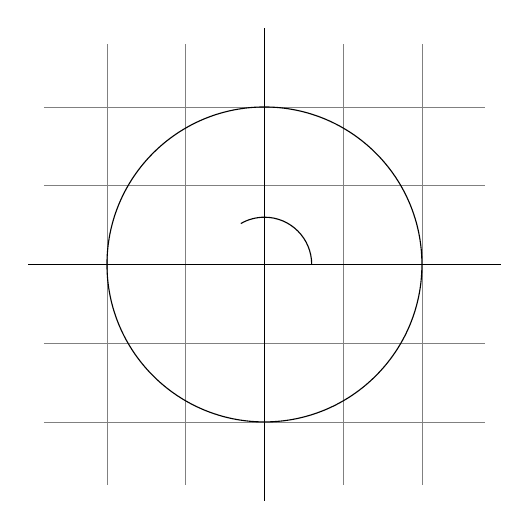
\begin{tikzpicture}[scale = 2]
    \draw[step=.5cm,gray,very thin] (-1.4,-1.4) grid (1.4,1.4);
    \draw (-1.5,0) -- (1.5,0);
    \draw (0,-1.5) -- (0,1.5);
    \draw (0,0) circle (1cm);
    \draw (3mm,0mm) arc (0:120:3mm);
\end{tikzpicture}
\end{cverbatim}

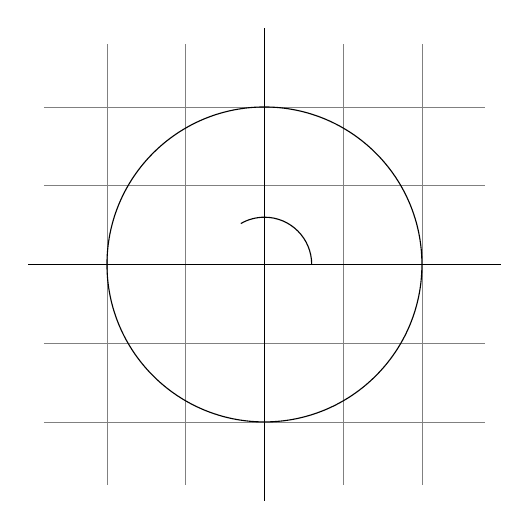
\begin{tikzpicture}[scale = 2]
    \draw[step=.5cm,gray,very thin] (-1.4,-1.4) grid (1.4,1.4);
    \draw (-1.5,0) -- (1.5,0);
    \draw (0,-1.5) -- (0,1.5);
    \draw (0,0) circle (1cm);
    \draw (3mm,0mm) arc (0:120:3mm);
\end{tikzpicture}

\begin{cverbatim}
\tikz \draw (0,0) arc (0:300:1.5cm and 1cm);
\end{cverbatim}

\tikz \draw (0,0) arc (0:300:1.5cm and 1cm);

\begin{cverbatim}
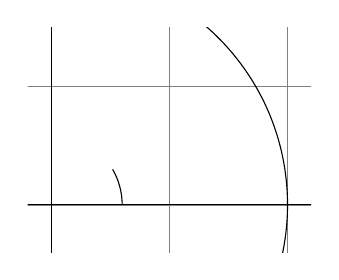
\begin{tikzpicture}[scale=3]
    \clip (-0.1,-0.2) rectangle (1.1,0.75);
    \draw[step=.5cm,gray,very thin] (-1.4,-1.4) grid (1.4,1.4);
    \draw (-1.5,0) -- (1.5,0);
    \draw (0,-1.5) -- (0,1.5);
    \draw (0,0) circle (1cm);
    \draw (3mm,0mm) arc (0:30:3mm);
\end{tikzpicture}
\end{cverbatim}

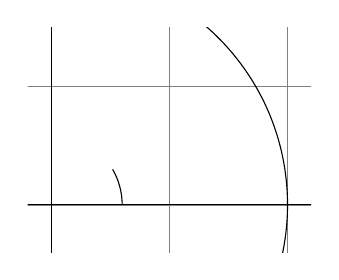
\begin{tikzpicture}[scale=3]
    \clip (-0.1,-0.2) rectangle (1.1,0.75);
    \draw[step=.5cm,gray,very thin] (-1.4,-1.4) grid (1.4,1.4);
    \draw (-1.5,0) -- (1.5,0);
    \draw (0,-1.5) -- (0,1.5);
    \draw (0,0) circle (1cm);
    \draw (3mm,0mm) arc (0:30:3mm);
\end{tikzpicture}

\begin{cverbatim}
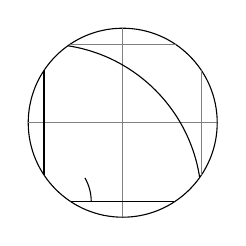
\begin{tikzpicture}[scale=2]
    \clip[draw] (0.5,0.5) circle (.6cm);
    \draw[step=.5cm,gray,very thin] (-1.4,-1.4) grid (1.4,1.4);
    \draw (-1.5,0) -- (1.5,0);
    \draw (0,-1.5) -- (0,1.5);
    \draw (0,0) circle (1cm);
    \draw (3mm,0mm) arc (0:30:3mm);
\end{tikzpicture}
\end{cverbatim}

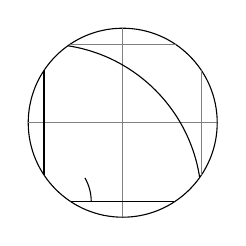
\begin{tikzpicture}[scale=2]
    \clip[draw] (0.5,0.5) circle (.6cm);
    \draw[step=.5cm,gray,very thin] (-1.4,-1.4) grid (1.4,1.4);
    \draw (-1.5,0) -- (1.5,0);
    \draw (0,-1.5) -- (0,1.5);
    \draw (0,0) circle (1cm);
    \draw (3mm,0mm) arc (0:30:3mm);
\end{tikzpicture}

\begin{cverbatim}
A sine \tikz \draw[x=1ex,y=1ex] 
            (0,0) sin (2,1) cos (4,0) sin (6,-1) cos (8,0);
 curve.
\end{cverbatim}

A sine \tikz \draw[x=1ex,y=1ex] 
            (0,0) sin (2,1) cos (4,0) sin (6,-1) cos (8,0);
 curve.

\begin{cverbatim}
\tikz \draw (0,0) sin (1,1) cos (2,0) sin (3,-1) cos (4,0)
            (0,1) cos (1,0) sin (2,-1) cos (3,0) sin (4,1);
\end{cverbatim}

\tikz \draw (0,0) sin (1,1) cos (2,0) sin (3,-1) cos (4,0)
            (0,1) cos (1,0) sin (2,-1) cos (3,0) sin (4,1);

\begin{cverbatim}
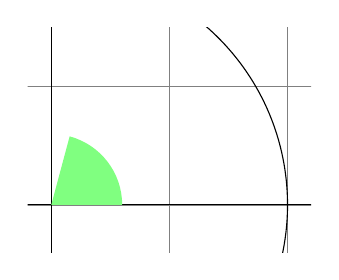
\begin{tikzpicture}[scale=3]
    \clip (-0.1,-0.2) rectangle (1.1,0.75);
    \draw[step=.5cm,gray,very thin] (-1.4,-1.4) grid (1.4,1.4);
    \draw (-1.5,0) -- (1.5,0);
    \draw (0,-1.5) -- (0,1.5);
    \draw (0,0) circle (1cm);
    \fill[green!50!white] (0,0) -- (3mm,0mm) arc (0:75:3mm) -- (0,0);
\end{tikzpicture}
\end{cverbatim}

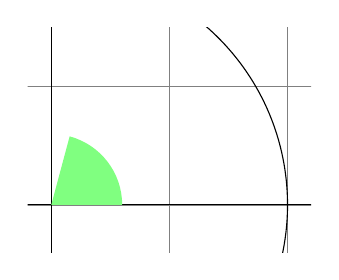
\begin{tikzpicture}[scale=3]
    \clip (-0.1,-0.2) rectangle (1.1,0.75);
    \draw[step=.5cm,gray,very thin] (-1.4,-1.4) grid (1.4,1.4);
    \draw (-1.5,0) -- (1.5,0);
    \draw (0,-1.5) -- (0,1.5);
    \draw (0,0) circle (1cm);
    \fill[green!50!white] (0,0) -- (3mm,0mm) arc (0:75:3mm) -- (0,0);
\end{tikzpicture}

\begin{cverbatim}
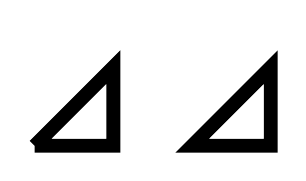
\begin{tikzpicture}[line width=5pt]
    \draw (0,0) -- (1,0) -- (1,1) -- (0,0);
    \draw (2,0) -- (3,0) -- (3,1) -- cycle; % cycle is better
    \useasboundingbox (0,1.5); % make bounding box higher
\end{tikzpicture}
\end{cverbatim}

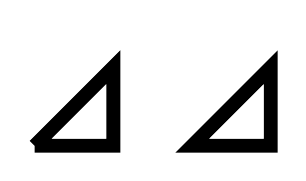
\begin{tikzpicture}[line width=5pt]
    \draw (0,0) -- (1,0) -- (1,1) -- (0,0);
    \draw (2,0) -- (3,0) -- (3,1) -- cycle; % cycle is better
    \useasboundingbox (0,1.5); % make bounding box higher
\end{tikzpicture}

\begin{cverbatim}
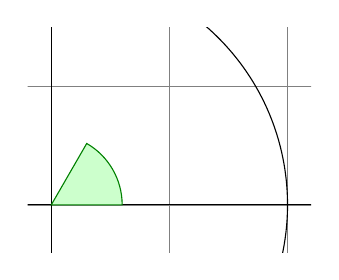
\begin{tikzpicture}[scale=3]
    \clip (-0.1,-0.2) rectangle (1.1,0.75);
    \draw[step=.5cm,gray,very thin] (-1.4,-1.4) grid (1.4,1.4);
    \draw (-1.5,0) -- (1.5,0);
    \draw (0,-1.5) -- (0,1.5);
    \draw (0,0) circle (1cm);
    \filldraw[fill=green!20!white, draw=green!50!black]
        (0,0) -- (3mm,0mm) arc (0:60:3mm) -- cycle;
\end{tikzpicture}
\end{cverbatim}

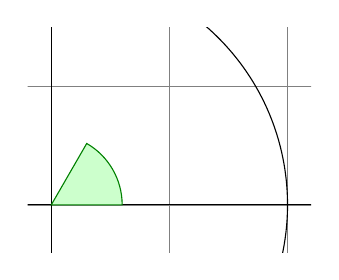
\begin{tikzpicture}[scale=3]
    \clip (-0.1,-0.2) rectangle (1.1,0.75);
    \draw[step=.5cm,gray,very thin] (-1.4,-1.4) grid (1.4,1.4);
    \draw (-1.5,0) -- (1.5,0);
    \draw (0,-1.5) -- (0,1.5);
    \draw (0,0) circle (1cm);
    \filldraw[fill=green!20!white, draw=green!50!black]
        (0,0) -- (3mm,0mm) arc (0:60:3mm) -- cycle;
\end{tikzpicture}

\begin{cverbatim}

\begin{tikzpicture}[rounded corners,ultra thick]
    \shade[top color=yellow,bottom color=black] (0,0) rectangle +(2,1);
    \shade[left color=yellow,right color=black] (3,0) rectangle +(2,1);
    \shadedraw[inner color=yellow,outer color=black,draw=yellow]
    (6,0) rectangle +(2,1);
    \shade[ball color=green] (9,.5) circle (.5cm);
\end{tikzpicture}
\end{cverbatim}


\begin{tikzpicture}[rounded corners,ultra thick]
    \shade[top color=yellow,bottom color=black] (0,0) rectangle +(2,1);
    \shade[left color=yellow,right color=black] (3,0) rectangle +(2,1);
    \shadedraw[inner color=yellow,outer color=black,draw=yellow]
    (6,0) rectangle +(2,1);
    \shade[ball color=green] (9,.5) circle (.5cm);
\end{tikzpicture}

\begin{cverbatim}
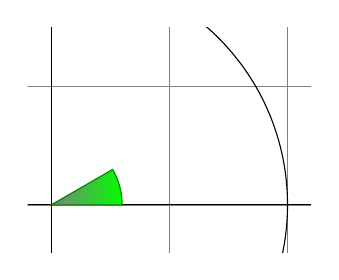
\begin{tikzpicture}[scale=3]
    \clip (-0.1,-0.2) rectangle (1.1,0.75);
    \draw[step=.5cm,gray,very thin] (-1.4,-1.4) grid (1.4,1.4);
    \draw (-1.5,0) -- (1.5,0);
    \draw (0,-1.5) -- (0,1.5);
    \draw (0,0) circle (1cm);
    \shadedraw[left color=gray,right color=green, draw=green!50!black]
        (0,0) -- (3mm,0mm) arc (0:30:3mm) -- cycle;
\end{tikzpicture}
\end{cverbatim}

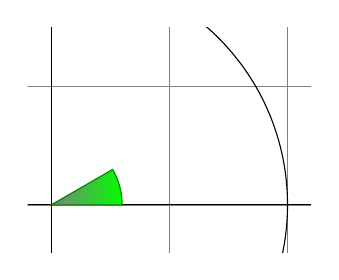
\begin{tikzpicture}[scale=3]
    \clip (-0.1,-0.2) rectangle (1.1,0.75);
    \draw[step=.5cm,gray,very thin] (-1.4,-1.4) grid (1.4,1.4);
    \draw (-1.5,0) -- (1.5,0);
    \draw (0,-1.5) -- (0,1.5);
    \draw (0,0) circle (1cm);
    \shadedraw[left color=gray,right color=green, draw=green!50!black]
        (0,0) -- (3mm,0mm) arc (0:30:3mm) -- cycle;
\end{tikzpicture}

\begin{cverbatim}
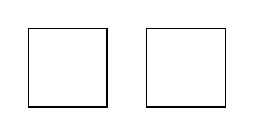
\begin{tikzpicture}
    % "++" local coordinates move with pen
    \def\rectanglepath{-- ++(1cm,0cm) -- ++(0cm,1cm) 
    -- ++(-1cm,0cm) --cycle}
    \draw (0,0) \rectanglepath;
    \draw (1.5,0) \rectanglepath;
\end{tikzpicture}
\end{cverbatim}

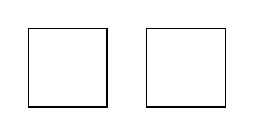
\begin{tikzpicture}
    \def\rectanglepath{-- ++(1cm,0cm) -- ++(0cm,1cm) 
    -- ++(-1cm,0cm) --cycle} % "++" -- local coordinates move with pen
    \draw (0,0) \rectanglepath;
    \draw (1.5,0) \rectanglepath;
\end{tikzpicture}

\begin{cverbatim}
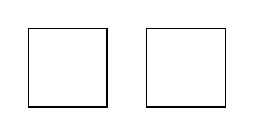
\begin{tikzpicture}
    \def\rectanglepath{-- +(1cm,0cm) -- +(1cm,1cm) -- +(0cm,1cm) -- cycle}
    \draw (0,0) \rectanglepath;
    \draw (1.5,0) \rectanglepath;
\end{tikzpicture}
\end{cverbatim}

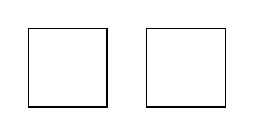
\begin{tikzpicture}
    \def\rectanglepath{-- +(1cm,0cm) -- +(1cm,1cm) -- +(0cm,1cm) -- cycle}
    \draw (0,0) \rectanglepath;
    \draw (1.5,0) \rectanglepath;
\end{tikzpicture}

\begin{cverbatim}
\begin{tikzpicture}[scale=3]
    \clip (-0.1,-0.2) rectangle (1.1,1.51);
    \draw[step=.5cm,gray,very thin] (-1.4,-1.4) grid (1.4,1.4);
    \draw[->] (-1.5,0) -- (1.5,0);
    \draw[->] (0,-1.5) -- (0,1.5);
    \draw (0,0) circle (1cm);
    \filldraw[fill=green!20,draw=green!50!black]
    (0,0) -- (3mm,0mm) arc (0:30:3mm) -- cycle;
    \draw[red,very thick] (30:1cm) -- +(0,-0.5);
    \draw[blue,very thick] (30:1cm) ++(0,-0.5) -- (0,0);

    \path [name path=upward line] (1,0) -- (1,1);
    \path [name path=sloped line] (0,0) -- (30:1.5cm);
    %find intersection of two invisible path
    \draw [name intersections={of=upward line and sloped line, by=x}]
          [very thick,orange] (1,0) -- (x);
\end{tikzpicture}
\end{cverbatim}

\begin{tikzpicture}[scale=3]
    \clip (-0.1,-0.2) rectangle (1.1,1.51);
    \draw[step=.5cm,gray,very thin] (-1.4,-1.4) grid (1.4,1.4);
    \draw[->] (-1.5,0) -- (1.5,0);
    \draw[->] (0,-1.5) -- (0,1.5);
    \draw (0,0) circle (1cm);
    \filldraw[fill=green!20,draw=green!50!black]
    (0,0) -- (3mm,0mm) arc (0:30:3mm) -- cycle;
    \draw[red,very thick] (30:1cm) -- +(0,-0.5);
    \draw[blue,very thick] (30:1cm) ++(0,-0.5) -- (0,0);

    \path [name path=upward line] (1,0) -- (1,1);
    \path [name path=sloped line] (0,0) -- (30:1.5cm);
    \draw [name intersections={of=upward line and sloped line, by=x}] %find intersection of two invisible path
          [very thick,orange] (1,0) -- (x);
\end{tikzpicture}


\begin{cverbatim}
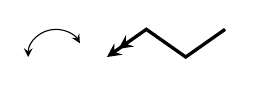
\begin{tikzpicture}[>=stealth]
    \draw [<->] (0,0) arc (180:30:10pt);
    \draw [<<-,very thick] (1,0) -- (1.5cm,10pt) 
    -- (2cm,0pt) -- (2.5cm,10pt);
\end{tikzpicture}
\end{cverbatim}

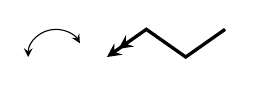
\begin{tikzpicture}[>=stealth]
    \draw [<->] (0,0) arc (180:30:10pt);
    \draw [<<-,very thick] (1,0) -- (1.5cm,10pt) 
    -- (2cm,0pt) -- (2.5cm,10pt);
\end{tikzpicture}

\begin{cverbatim}
\begin{tikzpicture}[ultra thick]
    \draw (0,0) -- (0,1);
    \begin{scope}[thin]
        \draw (1,0) -- (1,1);
        \draw (2,0) -- (2,1);
    \end{scope}
    \draw (3,0) -- (3,1);
\end{tikzpicture}
\end{cverbatim}

\begin{tikzpicture}[ultra thick]
    \draw (0,0) -- (0,1);
    \begin{scope}[thin]
        \draw (1,0) -- (1,1);
        \draw (2,0) -- (2,1);
    \end{scope}
    \draw (3,0) -- (3,1);
\end{tikzpicture}

\begin{cverbatim}
\tikz \draw (0,0) -- (0,0.5) [xshift=2pt] (0,0) -- (0,0.5);
\end{cverbatim}

\tikz \draw (0,0) -- (0,0.5) [xshift=2pt] (0,0) -- (0,0.5);

\begin{cverbatim}
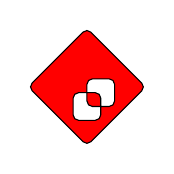
\begin{tikzpicture}[even odd rule,rounded corners=2pt,x=10pt,y=10pt]
    \filldraw[fill=red] (0,0) rectangle (1,1)
    [xshift=5pt,yshift=5pt] (0,0) rectangle (1,1)
    [rotate=45] (-1,-1) rectangle (2,2);
\end{tikzpicture}
\end{cverbatim}

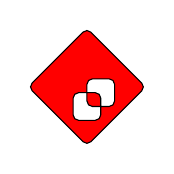
\begin{tikzpicture}[even odd rule,rounded corners=2pt,x=10pt,y=10pt]
    \filldraw[fill=red] (0,0) rectangle (1,1)
    [xshift=5pt,yshift=5pt] (0,0) rectangle (1,1)
    [rotate=45] (-1,-1) rectangle (2,2);
\end{tikzpicture}

\begin{cverbatim}
\tikz \foreach \x in {1,...,10}
        \draw (\x,0) circle (0.4cm);
\end{cverbatim}

\tikz \foreach \x in {1,...,10}
        \draw (\x,0) circle (0.4cm);

\begin{cverbatim}
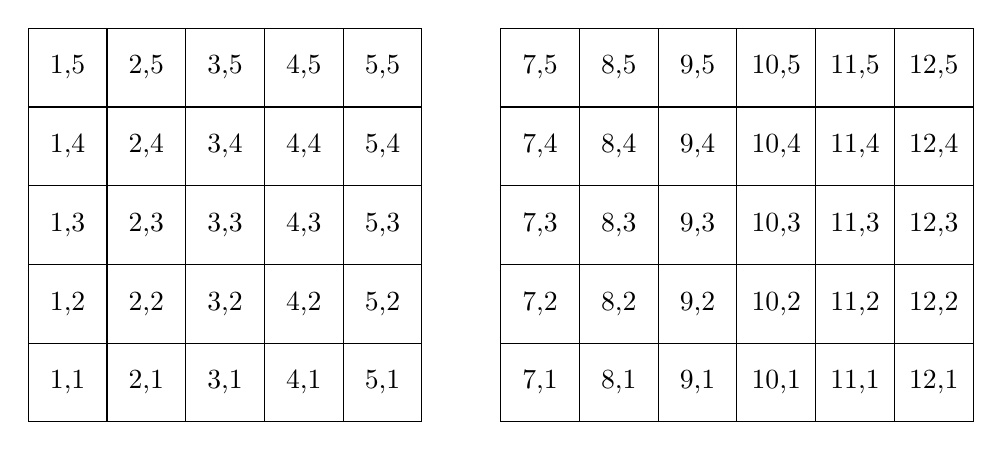
\begin{tikzpicture}
    \foreach \x in {1,2,...,5,7,8,...,12}
    \foreach \y in {1,...,5}
    {
        \draw (\x,\y) +(-.5,-.5) rectangle ++(.5,.5);
        \draw (\x,\y) node{\x,\y};
    }
\end{tikzpicture}
\end{cverbatim}

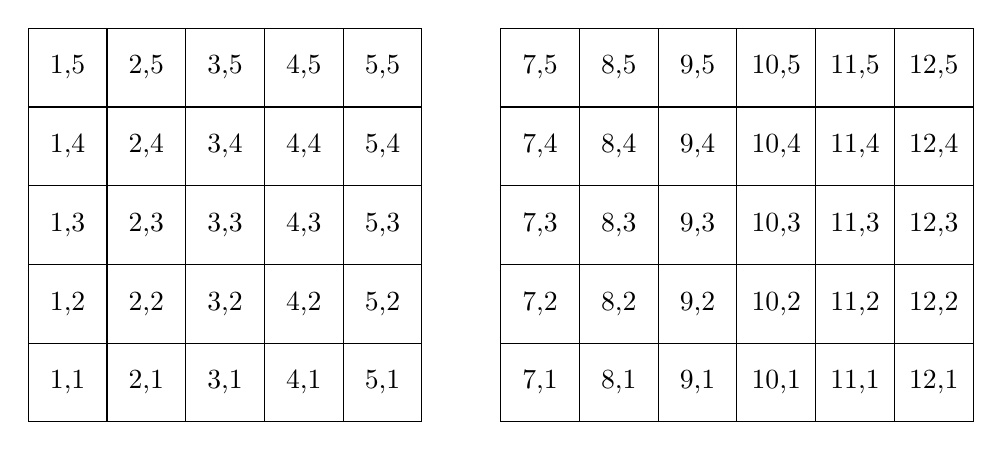
\begin{tikzpicture}
    \foreach \x in {1,2,...,5,7,8,...,12}
    \foreach \y in {1,...,5}
    {
        \draw (\x,\y) +(-.5,-.5) rectangle ++(.5,.5);
        \draw (\x,\y) node{\x,\y};
    }
\end{tikzpicture}

\begin{cverbatim}
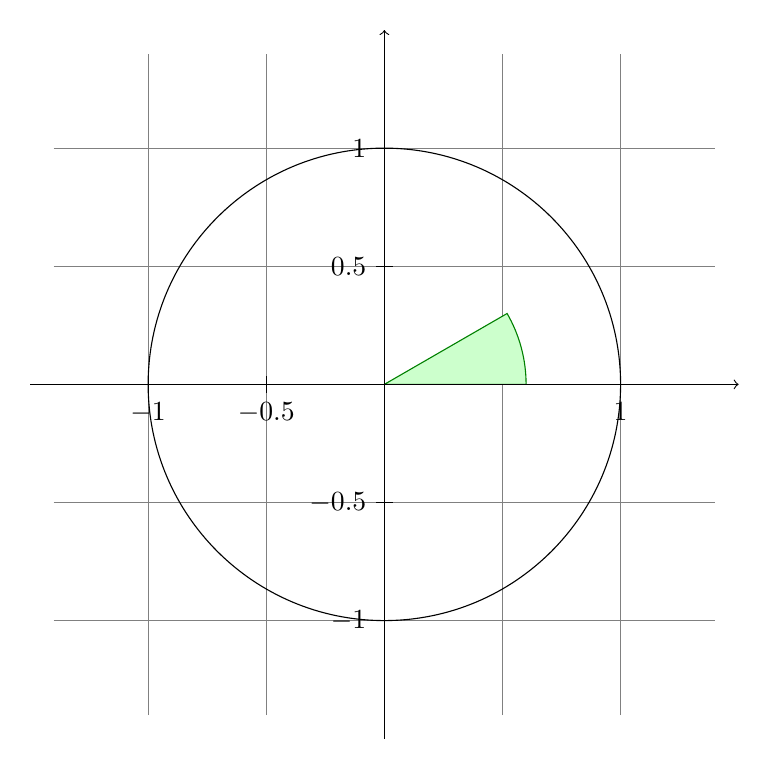
\begin{tikzpicture}[scale=3]
    \clip (-1.51,-1.51) rectangle (1.51,1.51);
    \draw[step=.5cm,help lines] (-1.4,-1.4) grid (1.4,1.4);
    \filldraw[fill=green!20,draw=green!50!black]
        (0,0) -- (6mm,0mm) arc (0:30:6mm) -- cycle;
    \draw[->] (-1.5,0) -- (1.5,0);
    \draw[->] (0,-1.5) -- (0,1.5);
    \draw (0,0) circle (1cm);
    \foreach \x in {-1,-0.5,1}
        \draw (\x cm,1pt) -- (\x cm,-1pt) node[anchor=north] {$\x$};
    \foreach \y in {-1,-0.5,0.5,1}
        \draw (1pt,\y cm) -- (-1pt,\y cm) node[anchor=east] {$\y$};
\end{tikzpicture}
\end{cverbatim}

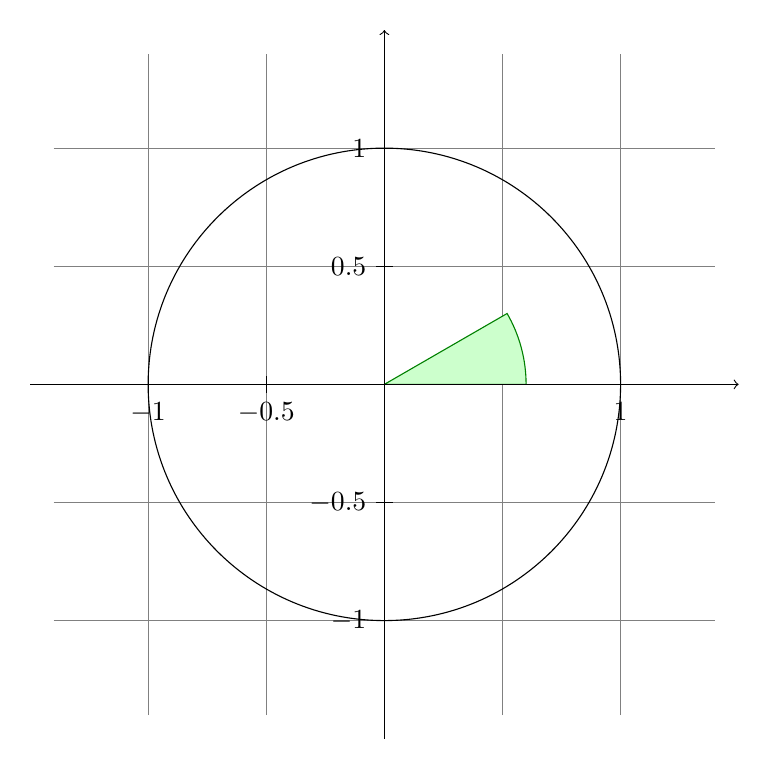
\begin{tikzpicture}[scale=3]
    \clip (-1.51,-1.51) rectangle (1.51,1.51);
    \draw[step=.5cm,help lines] (-1.4,-1.4) grid (1.4,1.4);
    \filldraw[fill=green!20,draw=green!50!black]
        (0,0) -- (6mm,0mm) arc (0:30:6mm) -- cycle;
    \draw[->] (-1.5,0) -- (1.5,0);
    \draw[->] (0,-1.5) -- (0,1.5);
    \draw (0,0) circle (1cm);
    \foreach \x in {-1,-0.5,1}
        \draw (\x cm,1pt) -- (\x cm,-1pt) node[anchor=north] {$\x$};
    \foreach \y in {-1,-0.5,0.5,1}
        \draw (1pt,\y cm) -- (-1pt,\y cm) node[anchor=east] {$\y$};
\end{tikzpicture}


\begin{cverbatim}
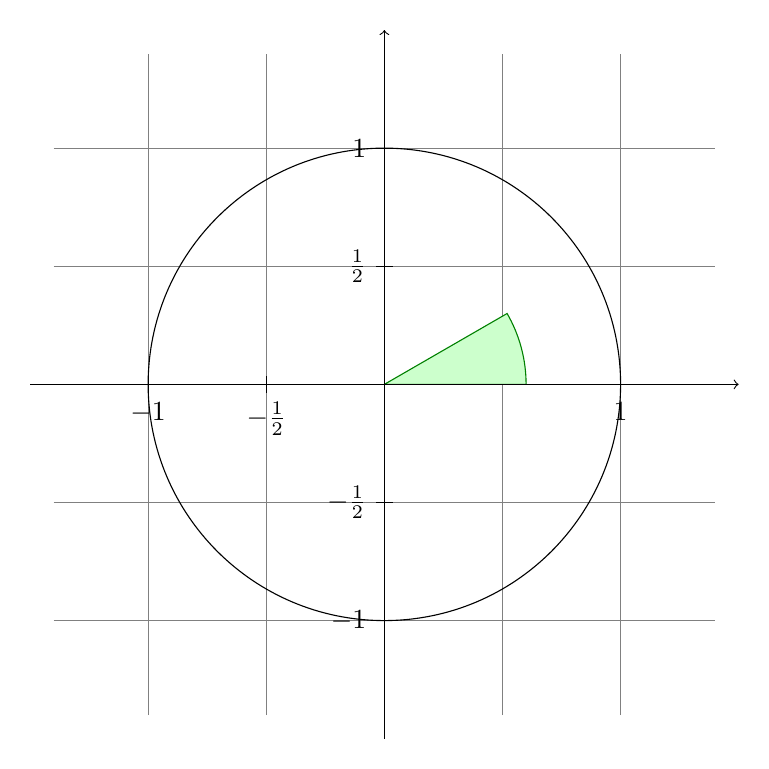
\begin{tikzpicture}[scale=3]
    \clip (-1.51,-1.51) rectangle (1.51,1.51);
    \draw[step=.5cm,help lines] (-1.4,-1.4) grid (1.4,1.4);
    \filldraw[fill=green!20,draw=green!50!black]
        (0,0) -- (6mm,0mm) arc (0:30:6mm) -- cycle;
    \draw[->] (-1.5,0) -- (1.5,0);
    \draw[->] (0,-1.5) -- (0,1.5);
    \draw (0,0) circle (1cm);
    \foreach \x/\xtext in {-1,-0.5/-\frac{1}{2},1}
        \draw (\x cm,1pt) -- (\x cm,-1pt) node[anchor=north] {$\xtext$};
    \foreach \y/\ytext in {-1,-0.5/-\frac{1}{2},0.5/\frac{1}{2},1}
        \draw (1pt,\y cm) -- (-1pt,\y cm) node[anchor=east] {$\ytext$};
\end{tikzpicture}
\end{cverbatim}

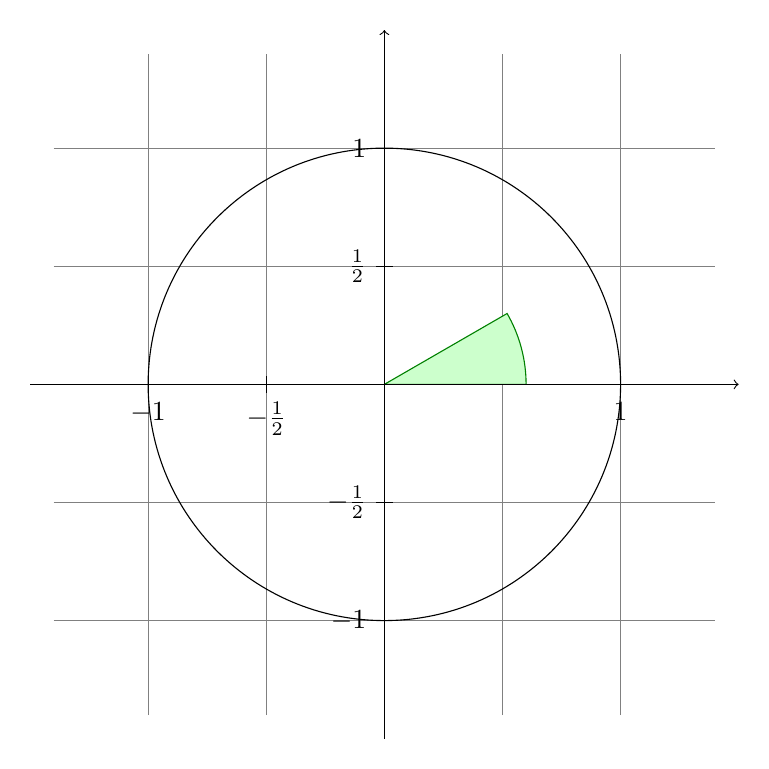
\begin{tikzpicture}[scale=3]
    \clip (-1.51,-1.51) rectangle (1.51,1.51);
    \draw[step=.5cm,help lines] (-1.4,-1.4) grid (1.4,1.4);
    \filldraw[fill=green!20,draw=green!50!black]
        (0,0) -- (6mm,0mm) arc (0:30:6mm) -- cycle;
    \draw[->] (-1.5,0) -- (1.5,0);
    \draw[->] (0,-1.5) -- (0,1.5);
    \draw (0,0) circle (1cm);
    \foreach \x/\xtext in {-1,-0.5/-\frac{1}{2},1}
        \draw (\x cm,1pt) -- (\x cm,-1pt) node[anchor=north] {$\xtext$};
    \foreach \y/\ytext in {-1,-0.5/-\frac{1}{2},0.5/\frac{1}{2},1}
        \draw (1pt,\y cm) -- (-1pt,\y cm) node[anchor=east] {$\ytext$};
\end{tikzpicture}

\begin{cverbatim}
\begin{tikzpicture}[scale=3]
    \draw[step=.5cm,gray,very thin] (-1.4,-1.4) grid (1.4,1.4);
    \filldraw[fill=green!20,draw=green!50!black] (0,0) -- (3mm,0mm) arc
    (0:30:3mm) -- cycle;
    \draw[->] (-1.5,0) -- (1.5,0) coordinate (x axis);
    \draw[->] (0,-1.5) -- (0,1.5) coordinate (y axis);
    \draw (0,0) circle (1cm);

    \draw[very thick,red]
    (30:1cm) -- node[left=1pt,fill=blue!20] {$\sin \alpha$} (30:1cm |- x axis);
    \draw[very thick,blue]
    (30:1cm |- x axis) -- node[below=2pt,fill=red!20] {$\cos \alpha$} (0,0);
    
    \path [name path=upward line] (1,0) -- (1,1);
    \path [name path=sloped line] (0,0) -- (30:1.5cm);
    \draw [name intersections={of=upward line and sloped line, by=t}]
    [very thick,orange] (1,0) -- node [right=1pt,fill=cyan!20]
    {$\displaystyle \tan \alpha \color{black}=
        \frac{{\color{red}\sin \alpha}}{\color{blue}\cos \alpha}$} (t);
    \draw (0,0) -- (t);

    \foreach \x/\xtext in {-1,-0.5/-\frac{1}{2},1}
        \draw (\x cm,1pt) -- (\x cm,-1pt) node[anchor=north] {$\xtext$};
    \foreach \y/\ytext in {-1,-0.5/-\frac{1}{2},0.5/\frac{1}{2},1}
        \draw (1pt,\y cm) -- (-1pt,\y cm) node[anchor=east] {$\ytext$};

\end{tikzpicture}
\end{cverbatim}

\begin{tikzpicture}[scale=3]
    \draw[step=.5cm,gray,very thin] (-1.4,-1.4) grid (1.4,1.4);
    \filldraw[fill=green!20,draw=green!50!black] (0,0) -- (3mm,0mm) arc
    (0:30:3mm) -- cycle;
    \draw[->] (-1.5,0) -- (1.5,0) coordinate (x axis);
    \draw[->] (0,-1.5) -- (0,1.5) coordinate (y axis);
    \draw (0,0) circle (1cm);

    \draw[very thick,red]
    (30:1cm) -- node[left=1pt,fill=blue!20] {$\sin \alpha$} (30:1cm |- x axis);
    \draw[very thick,blue]
    (30:1cm |- x axis) -- node[below=2pt,fill=red!20] {$\cos \alpha$} (0,0);
    
    \path [name path=upward line] (1,0) -- (1,1);
    \path [name path=sloped line] (0,0) -- (30:1.5cm);
    \draw [name intersections={of=upward line and sloped line, by=t}]
    [very thick,orange] (1,0) -- node [right=1pt,fill=cyan!20]
    {$\displaystyle \tan \alpha \color{black}=
        \frac{{\color{red}\sin \alpha}}{\color{blue}\cos \alpha}$} (t);
    \draw (0,0) -- (t);

    \foreach \x/\xtext in {-1,-0.5/-\frac{1}{2},1}
        \draw (\x cm,1pt) -- (\x cm,-1pt) node[anchor=north] {$\xtext$};
    \foreach \y/\ytext in {-1,-0.5/-\frac{1}{2},0.5/\frac{1}{2},1}
        \draw (1pt,\y cm) -- (-1pt,\y cm) node[anchor=east] {$\ytext$};

\end{tikzpicture}

\begin{cverbatim}
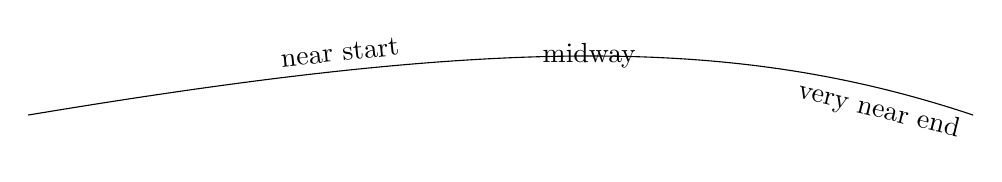
\begin{tikzpicture}
    \draw (0,0) .. controls (6,1) and (9,1) ..
    node[near start,sloped,above] {near start}
    node {midway}
    node[very near end,sloped,below] {very near end} (12,0);
\end{tikzpicture}
\end{cverbatim}

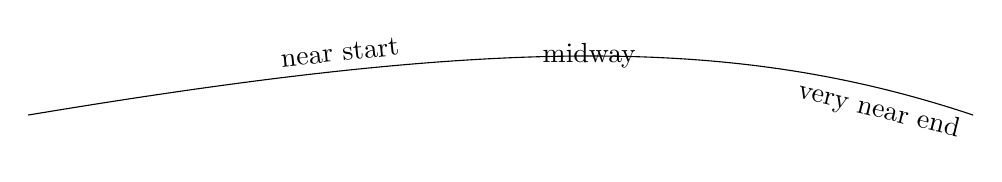
\begin{tikzpicture}
    \draw (0,0) .. controls (6,1) and (9,1) ..
    node[near start,sloped,above] {near start}
    node {midway}
    node[very near end,sloped,below] {very near end} (12,0);
\end{tikzpicture}



\begin{cverbatim}
\begin{tikzpicture}
    [scale=3,line cap=round,
    % Styles
    axes/.style=,
    important line/.style={very thick},
    information text/.style={rounded corners,fill=red!10,inner sep=1ex}]
    % Local definitions
    \def\costhirty{0.8660256}
    % Colors
    \colorlet{anglecolor}{green!50!black}
    \colorlet{sincolor}{red}
    \colorlet{tancolor}{orange!80!black}
    \colorlet{coscolor}{blue}
    % The graphic
    \draw[help lines,step=0.5cm] (-1.4,-1.4) grid (1.4,1.4);
    \draw (0,0) circle (1cm);
    \begin{scope}[axes]
        \draw[->] (-1.5,0) -- (1.5,0) node[right] {$x$} coordinate(x axis);
        \draw[->] (0,-1.5) -- (0,1.5) node[above] {$y$} coordinate(y axis);
        \foreach \x/\xtext in {-1, -.5/-\frac{1}{2}, 1}
        \draw[xshift=\x cm] (0pt,1pt) -- (0pt,-1pt) node[below,fill=white] {$\xtext$};
        \foreach \y/\ytext in {-1, -.5/-\frac{1}{2}, .5/\frac{1}{2}, 1}
        \draw[yshift=\y cm] (1pt,0pt) -- (-1pt,0pt) node[left,fill=white] {$\ytext$};
    \end{scope}
    \filldraw[fill=green!20,draw=anglecolor] (0,0) -- (3mm,0pt) arc(0:30:3mm);
    \draw (15:2mm) node[anglecolor] {$\alpha$};
    \draw[important line,sincolor]
    (30:1cm) -- node[left=1pt,fill=white] {$\sin \alpha$} (30:1cm |- x axis);
    \draw[important line,coscolor]
    (30:1cm |- x axis) -- node[below=2pt,fill=white] {$\cos \alpha$} (0,0);
    \path [name path=upward line] (1,0) -- (1,1);
    \path [name path=sloped line] (0,0) -- (30:1.5cm);
    \draw [name intersections={of=upward line and sloped line, by=t}]
    [very thick,orange] (1,0) -- node [right=1pt,fill=white]
    {$\displaystyle \tan \alpha \color{black}=
        \frac{{\color{red}\sin \alpha}}{\color{blue}\cos \alpha}$} (t);
    \draw (0,0) -- (t);
    \draw[xshift=2.0cm]
    node[right,text width=6cm,information text]
    {
        The {\color{anglecolor} angle $\alpha$} is $30^\circ$ in the
        example ($\pi/6$ in radians). The {\color{sincolor}sine of
            $\alpha$}, which is the height of the red line, is
        \[
            {\color{sincolor} \sin \alpha} = 1/2.
        \]
        By the Theorem of Pythagoras ...
    };
\end{tikzpicture}
\end{cverbatim}

\begin{tikzpicture}
    [scale=3,line cap=round,
    % Styles
    axes/.style=,
    important line/.style={very thick},
    information text/.style={rounded corners,fill=red!10,inner sep=1ex}]
    % Local definitions
    \def\costhirty{0.8660256}
    % Colors
    \colorlet{anglecolor}{green!50!black}
    \colorlet{sincolor}{red}
    \colorlet{tancolor}{orange!80!black}
    \colorlet{coscolor}{blue}
    % The graphic
    \draw[help lines,step=0.5cm] (-1.4,-1.4) grid (1.4,1.4);
    \draw (0,0) circle (1cm);
    \begin{scope}[axes]
        \draw[->] (-1.5,0) -- (1.5,0) node[right] {$x$} coordinate(x axis);
        \draw[->] (0,-1.5) -- (0,1.5) node[above] {$y$} coordinate(y axis);
        \foreach \x/\xtext in {-1, -.5/-\frac{1}{2}, 1}
        \draw[xshift=\x cm] (0pt,1pt) -- (0pt,-1pt) node[below,fill=white] {$\xtext$};
        \foreach \y/\ytext in {-1, -.5/-\frac{1}{2}, .5/\frac{1}{2}, 1}
        \draw[yshift=\y cm] (1pt,0pt) -- (-1pt,0pt) node[left,fill=white] {$\ytext$};
    \end{scope}
    \filldraw[fill=green!20,draw=anglecolor] (0,0) -- (3mm,0pt) arc(0:30:3mm);
    \draw (15:2mm) node[anglecolor] {$\alpha$};
    \draw[important line,sincolor]
    (30:1cm) -- node[left=1pt,fill=white] {$\sin \alpha$} (30:1cm |- x axis);
    \draw[important line,coscolor]
    (30:1cm |- x axis) -- node[below=2pt,fill=white] {$\cos \alpha$} (0,0);
    \path [name path=upward line] (1,0) -- (1,1);
    \path [name path=sloped line] (0,0) -- (30:1.5cm);
    \draw [name intersections={of=upward line and sloped line, by=t}]
    [very thick,orange] (1,0) -- node [right=1pt,fill=white]
    {$\displaystyle \tan \alpha \color{black}=
        \frac{{\color{red}\sin \alpha}}{\color{blue}\cos \alpha}$} (t);
    \draw (0,0) -- (t);
    \draw[xshift=2.0cm]
    node[right,text width=6cm,information text]
    {
        The {\color{anglecolor} angle $\alpha$} is $30^\circ$ in the
        example ($\pi/6$ in radians). The {\color{sincolor}sine of
            $\alpha$}, which is the height of the red line, is
        \[
            {\color{sincolor} \sin \alpha} = 1/2.
        \]
        By the Theorem of Pythagoras ...
    };
\end{tikzpicture}

